\newpage
\section{Математика}
\subsection{Системы координат}
\label{sec:coord-systems}

\begin{wrapfigure}{r}{0.27\tw}
    \centering
    \vspace{-1pc}
    \tikzsetnextfilename{math-coord-sys-decart}
    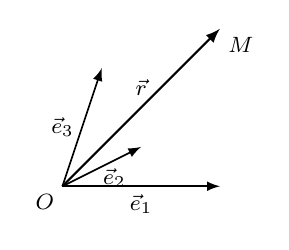
\begin{tikzpicture}[scale=1]
        \footnotesize
        \coordinate (O) at (0, 0);
        \coordinate (E1) at (2, 0);
        \coordinate (E2) at (1, 0.5);
        \coordinate (E3) at (0.5, 1.5);
        \coordinate (M) at (2, 2);

        \draw[semithick, -latex] (O) -- (E1);
        \draw[semithick, -latex] (O) -- (E2);
        \draw[semithick, -latex] (O) -- (E3);
        \draw[thick, -latex] (O) -- (M);

        \point (O);
        \point (M);

        \draw (1, 0) node[anchor=north]{$\vec{e}_1$};
        \draw (0.66, 0.33) node[anchor=north]{$\vec{e}_2$};
        \draw (0.25, 0.75) node[anchor=east]{$\vec{e}_3$};
        \draw (1, 1.05) node[anchor=south]{$\vec{r}$};
        \draw (M) node[anchor=north west]{$M$};
        \draw (O) node[anchor=north east]{$O$};
    \end{tikzpicture}
    \caption{}
    \vspace{-1pc}
    \label{pic:math-coord-sys-decart}
\end{wrapfigure}
Зафиксируем точку $O$ в пространстве и рассмотрим произвольную точку $M$. Вектор $\vec{r} = \overrightarrow{OM}$ называется радиус-вектором точки $M$. Пусть в рассматриваемом пространстве также выбран базис $\{\vec{e}_1, \ldots, \vec{e}_n \}$, тогда совокупность точка $O$ и базиса называется \term{декартовой системой координат}. Причем точка $O$~--- начало координат, а базисные векторы $\vec{e}_1, \ldots, \vec{e}_n$ задают координатные оси.

\begin{wrapfigure}{r}{0.27\tw}
    \centering
    \vspace{-1pc}
    \tikzsetnextfilename{math-coord-sys-ord-basis}
    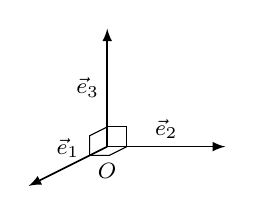
\begin{tikzpicture}[scale=1]
        \footnotesize
        \coordinate (O) at (0, 0);
        \coordinate (E1) at (1.5, 0);
        \coordinate (E2) at (-1, -0.5);
        \coordinate (E3) at (0, 1.5);
%        \coordinate (M) at (2, 2);

        \draw[semithick, -latex] (O) -- (E1);
        \draw[semithick, -latex] (O) -- (E2);
        \draw[semithick, -latex] (O) -- (E3);
%        \draw[thick, -latex] (O) -- (M);

        \point (O);
%        \point (M);

        \draw (-0.5, -0.25) node[anchor=south]{$\vec{e}_1$};
        \draw (0.75, 0) node[anchor=south]{$\vec{e}_2$};
        \draw (0, 0.75) node[anchor=east]{$\vec{e}_3$};
%        \draw (1, 1.05) node[anchor=south]{$\vec{r}$};
%        \draw (M) node[anchor=south]{$M$};
        \draw (0, -0.1) node[anchor=north]{$O$};

        \draw (0, 0.25) -- (0.25, 0.25) -- (0.25, 0);
        \draw (0.25, 0) -- (0.027, -0.112) -- (-0.223, -0.112);
        \draw (0, 0.25) -- (-0.223, 0.138) -- (-0.223, -0.112);
    \end{tikzpicture}
    \caption{}
    \vspace{-1pc}
    \label{pic:math-coord-sys-ord-basis}
\end{wrapfigure}
Однако пользоваться представлением векторов в произвольном базисе довольно сложно, поэтому рассмотрим специальный тип~--- \term{орто\-нор\-ми\-рованный базис}~--- это такой базис, базисные векторы которого попарно ортогональны, и длина каждого равна единице.

\term{Прямоугольной декартовой системой координат} (ПДСК) называют декартову систему координат с ортонормированным базисом. В практических задачах использовать ПДСК не всегда удобно, поэтому также рассмотрим другие системы координат. 

\begin{wrapfigure}{r}{0.27\tw}
    \centering
    \vspace{-1pc}
    \tikzsetnextfilename{math-coord-sys-polar}
    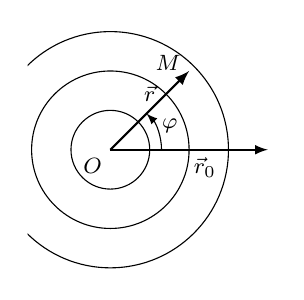
\begin{tikzpicture}[scale=1]
        \clip(-1.05, -1.55) rectangle (2.1, 1.55);

        \footnotesize
        \coordinate (O) at (0, 0);
        \coordinate (E1) at (2, 0);
%        \coordinate (E2) at (1, 0.5);
%        \coordinate (E3) at (0.5, 1.5);
        \coordinate (M) at (1, 1);

        \draw[semithick, -latex] (O) -- (E1);
%        \draw[semithick, -latex] (O) -- (E2);
%        \draw[semithick, -latex] (O) -- (E3);
        \draw[thick, -latex] (O) -- (M);
        \draw[-latex] (0.65, 0) arc(0:45:0.65);

        \foreach \r in {0.5, 1, 1.5} {
            \draw (O) circle(\r);
        };

        \point (O);
        \point (M);

        \draw (1.2, 0) node[anchor=north]{$\vec{r}_0$};
%        \draw (0.66, 0.33) node[anchor=north]{$\vec{e}_2$};
%        \draw (0.25, 0.75) node[anchor=east]{$\vec{e}_3$};
        \draw (0.5, 0.5) node[anchor=south]{$\vec{r}$};
        \draw (0.55, 0.3) node[anchor=west]{$\varphi$};
        \draw (1, 0.9) node[anchor=south east]{$M$};
        \draw (O) node[anchor=north east]{$O$};
    \end{tikzpicture}
    \caption{}
    \label{pic:math-coord-sys-polar}
\end{wrapfigure}
На плоскости, то есть в пространстве $\R^2$, имеющем размерность два, часто применяется \term{полярная система координат}. В ней координатами вектора является его длина $r$~--- расстояние до точки от начала отсчёта, и угол $\varphi$ радиус-вектора с начальной ось.

Пусть $(x,y)$~--- координаты некоторого вектора в ПДСК на $\R^2$, тогда не сложно получить, что его координаты в полярной системе координат (начальная ось совпадает с осью $Ox$)  удовлетворяют следующим соотношениям:
\begin{equation}
    \begin{cases}
        r = \sqrt{x^2 + y^2},\\
        \sin \varphi = y/r,\\
        \cos \varphi = x/r.
    \end{cases}
    \quad \Leftrightarrow \quad
    \begin{cases}
        x = r \cos \varphi,\\
        y = r \sin \varphi.
    \end{cases}
\end{equation}

\begin{wrapfigure}{r}{0.35\tw}
    \centering
%    \vspace{-1pc}
    \tikzsetnextfilename{math-coord-sys-cyl}
    \begin{tikzpicture}[scale=1]
        \clip(-1.3, -1.1) rectangle (2.5, 2.5);

        \footnotesize
        \coordinate (O) at (0, 0);
        \coordinate (E1) at (2.3, 0);
        \coordinate (E2) at (0, 2.3);
        \coordinate (E3) at (-1, -1);
        \coordinate (M) at (0.8, 1.3);
        \coordinate (M') at (0.8, -0.48);
        \coordinate (M'') at (1, -0.6);

        \draw[semithick, -latex] (O) -- (E1);
        \draw[semithick, -latex] (O) -- (E2);
        \draw[semithick, -latex] (O) -- (E3);
        \draw[thick, -latex] (O) -- (M);

        \draw [dashes] (0, 1.78) -- (M) -- (M');
        \draw [dashes] (M'') -- (O);
        \draw [dashes] (1.28, 0) -- (M') -- (-0.48, -0.48);

        \draw (O) ellipse(2 and 0.7);
        \draw (0, 1.78) ellipse(2 and 0.7);

        \draw [-latex](-0.2, -0.2) arc(-99.4:-75.76:1.22);

        \foreach \p in {O, M, M', M''} {
            \point (\p);
        };

        \draw (0.5, 0.65) node[anchor=south east]{$\vec{r}$};
        \draw (0.05, -0.15) node[anchor=north]{$\varphi$};
        \draw (0.42, -0.2) node[anchor=west]{$r$};
        \draw (0.8, 0.4) node[anchor=west]{$h$};
        \draw (M) node[anchor=south west]{$M$};
        \draw (O) node[anchor=south east]{$O$};

        \draw (E1) node[anchor=north]{$y$};
        \draw (E2) node[anchor=east]{$z$};
        \draw (E3) node[anchor=east]{$x$};
    \end{tikzpicture}
    \caption{}
    \label{pic:math-coord-sys-cyl}
    \vspace{-2pc}
\end{wrapfigure}
Теперь пусть $(x, y, z)$~--- координаты некоторого вектора в ПДСК на~$\R^3$. Обозначим за $h$~--- длину проекции этого вектора на ось $z$, $r$~--- длину его проекции на плоскость $Oxy$, $\varphi$~--- угол между проекцией на плоскость $Oxy$ и осью $Ox$. Тогда тройка $(r, \varphi, h)$~--- координаты рассматриваемого векторы в \term{цилиндрической системе координат}, и верно представление
\begin{equation}
    \begin{cases}
        r = \sqrt{x^2 + y^2},\\
        \sin \varphi = y/r,\\
        \cos \varphi = x/r,\\
        h = z.
    \end{cases}
    \quad \Leftrightarrow \quad
    \begin{cases}
        x = r \cos \varphi,\\
        y = r \sin \varphi,\\
        z = h.
    \end{cases}
\end{equation}

\begin{wrapfigure}{r}{0.35\tw}
    \centering
    \vspace{-2.5pc}
    \tikzsetnextfilename{math-coord-sys-sphere}
    \begin{tikzpicture}[scale=1]
        \clip(-1.3, -1.1) rectangle (2.5, 2.5);

        \footnotesize
        \coordinate (O) at (0, 0);
        \coordinate (E1) at (2.3, 0);
        \coordinate (E2) at (0, 2.3);
        \coordinate (E3) at (-1, -1);
        \coordinate (M) at (0.8, 1.3);
        \coordinate (M') at (0.8, -0.48);
        \coordinate (M'') at (1, -0.6);

        \draw[semithick, -latex] (O) -- (E1);
        \draw[semithick, -latex] (O) -- (E2);
        \draw[semithick, -latex] (O) -- (E3);
        \draw[thick, -latex] (O) -- (M);

        \draw [dashes] (0, 1.78) -- (M) -- (M');
        \draw [dashes] (M'') -- (O);
        \draw [dashes] (0, 2) arc(90:-90:1.05 and 2);
        \draw [dashes] (M') -- (-0.48, -0.48);
        \draw [dashes] (M') -- (1.28, 0);
%        \draw[-latex] (1.02, 0) arc(0:45:1 and 0.4);

        \draw (O) circle(2);
        \draw (0, 2) arc(90:270:0.7 and 2);
        \draw (2, 0) arc(360:180:2 and 0.7);

        \draw [-latex](-0.2, -0.2) arc(-99.4:-75.76:1.22);
        \draw [-latex](0.29, -0.18) arc(-9.44:18:1.22);
%        \draw (O) ellipse(0.6 and 0.21);
%        \draw (-1, 0) circle(1.3);


        \foreach \p in {O, M, M', M''} {
            \point (\p);
        };


        \draw (0.5, 0.6) node[anchor=south east]{$\vec{r}$};
%        \draw (1.05, -0.25) node[anchor=west]{$x$};
%        \draw (0.2, -0.45) node[anchor=north]{$y$};
%        \draw (0.75, 0.3) node[anchor=west]{$z$};
        \draw (0.3, 0.15) node[anchor=west]{$\varphi$};
        \draw (0.05, -0.15) node[anchor=north]{$\theta$};
        \draw (M) node[anchor=west]{$M$};
        \draw (O) node[anchor=south east]{$O$};

        \draw (E1) node[anchor=north]{$y$};
        \draw (E2) node[anchor=east]{$z$};
        \draw (E3) node[anchor=east]{$x$};
    \end{tikzpicture}
    \caption{}
    \label{pic:math-coord-sys-sphere}
    \vspace{-1.5pc}
\end{wrapfigure}
Остается рассмотреть \term{сферическую систему координат}. Здесь координатами точки будет длина $r$ радиус-вектора $\vec{r}$ и два угла: $\theta$~--- угол между радиус-вектором и плоскостью $Oxy$ и $\varphi$~--- угол между проекцией радиус-вектора на плоскость $Oxy$ и осью $Ox$. Верны формулы перехода:
\begin{equation}
    \begin{cases}
        r = \sqrt{x^2 + y^2 + z^2},\\
        \theta = \arcsin{z/r},\\
        \sin \varphi = y/r,\\
        \cos \varphi = x/r.
    \end{cases}
    \quad \Leftrightarrow \quad
    \begin{cases}
        x = r \cos \theta \cos \varphi    ,\\
        y = r \cos \theta \sin \varphi,\\
        z = r \sin \theta.
    \end{cases}
\end{equation}

\subsection{Скалярное произведение}
\term{Скалярным произведением} двух векторов называется билинейная операция над ними, зависящая только от длин этих векторов и угла между ними, результатом которой является скаляр. Скалярное произведение векторов $\vec{a}$ и  $\vec{b}$ выражается следующим образом:
\begin{equation}
    \scalar{a}{b} = |\vec{a}||\vec{b}| \cos \widehat{\vec{a}\vec{b}}. \label{eq:scalar-prod1}
\end{equation}
\begin{equation}
    \scalar{a}{b} = \vec{a}^{\T} \vec{b} =
    \begin{pmatrix}
        a_1 & \cdots & a_n
    \end{pmatrix}
    \begin{pmatrix}
        b_1\\
        \vdots\\
        b_n
    \end{pmatrix}
    = a_1 b_1 + \ldots + a_n b_n.
    \label{eq:scalar-prod2}
\end{equation}

Докажем эквивалентность \eqref{eq:scalar-prod1} и \eqref{eq:scalar-prod2}. Пусть в ортонормированном базисе $\{\vec{e}_1, \ldots, \vec{e}_2\}$ векторы имеют следующие представления:
\begin{equation}
    \vec{a} = \sum\limits_{i = 1}^n a_i \vec{e}_i, \qquad \vec{b} = \sum\limits_{i = 1}^n b_i \vec{e}_i.
\end{equation}
Заметим, что $(\vec{a} \cdot \vec{e}_i) = |\vec{a}||\vec{e}_i| \cos \theta_i = |\vec{a}| \cos \theta_i = a_i$, где $\theta_i$~--- угол вектора $\vec{a}$ с $i$-м базисным вектором $\vec{e}_i$. Тогда
\begin{equation}
    \scalar{a}{b} = \left( \vec{a} \cdot \sum\limits_{i=1}^n b_i\vec{e}_i \right) = \sum\limits_{i=1}^n b_i(\vec{a} \cdot \vec{e}_i) = \sum\limits_{i=1}^n a_i b_i = a^{\T}b.
\end{equation}

Из \eqref{eq:scalar-prod1} и \eqref{eq:scalar-prod2} очевидна билинейность и симметричность скалярного произведение, то есть
\begin{equation}
    \scalar{(a + b)}{(c + d)} = \scalar{(c + d)}{(a + b)} = \scalar{a}{c} + \scalar{a}{d} + \scalar{b}{c} + \scalar{b}{d}.
\end{equation}

Практическое пременение скалярное произведение находит в вопросах проверки ортогональности векторов (как частный случай нахождения угла между векторами), потому что $\vec{a} \perp \vec{b}$ тогда и только тогда, когда $\scalar{a}{b} = 0$, так как
\begin{equation}
    \cos \widehat{\vec{a}\vec{b}} = \frac{\scalar{a}{b}}{|\vec{a}||\vec{b}|}.
\end{equation}

Отсюда также получается выражение для проекции вектора $\vec{a}$ на прямую с направляющим вектором $\vec{l}$:
\begin{equation}
    \pr_\vec{l} \vec{a} = \frac{\scalar{a}{l}}{|\vec{l}|^2} \vec{l}.
\end{equation}

Используя скалярное произведение, получим важную утверждение теоремы косинусов из планиметрии: пусть $\vec{c} = \vec{b} - \vec{a}$, то есть имеем треугольник со сторонами $|\vec{a}|$, $|\vec{b}|$ и $|\vec{c}|$. Рассмотрим скалярное произведение вектора $\vec{c}$ самого на себя:
\begin{multline}
    \scalar{c}{c} = \scalar{(b - a)}{(b - a)} = \scalar{b}{(b-a)} - \scalar{a}{(b - a)} = \\
    = \scalar{b}{b} - 2\scalar{b}{a} + \scalar{a}{a}
\end{multline}
\begin{equation}
    c^2 = b^2 + a^2 - 2ab\cos \widehat{\vec{a}\vec{b}}
\end{equation}

\subsection{Векторное произведение}
\label{sec:cross-product}

Тройку векторов будем называть \imp{правой}, если для наблюдателя, находящегося в конце третьего вектора, кратчайший поворот от первого вектора ко второму осуществляется против часовой стрелки, иначе левой.

Рассмотрим еще одну операцию над векторами~--- \term{векторное произведение} $\cross{a}{b}: \R^3 \times \R^3 \rightarrow \R^3$~--- антисимметричную и билинейную, задаваемую по правилу:
\begin{equation}
    \cross{a}{b} = |\vec{a}||\vec{b}| \sin \widehat{\vec{a}\vec{b}} \cdot \vec{n},
\end{equation}
\begin{wrapfigure}{r}{0.25\tw}
    \centering
    \vspace{.1pc}
    \tikzsetnextfilename{math-cross}
    \begin{tikzpicture}[scale=1]
        \footnotesize
        \coordinate (O) at (0, 0);
        \coordinate (A) at (1.5, 0);
        \coordinate (B) at (1, 0.5);
        \coordinate (AB) at (2.5, 0.5);
        \coordinate (N) at (0, 1.5);

        \draw[thick, -latex] (O) -- (A);
        \draw[thick, -latex] (O) -- (B);
        \draw[semithick, -latex] (O) -- (N);

        \draw[dashes] (A) -- (AB);
        \draw[dashes] (B) -- (AB);

        \draw (0.75, 0) node[anchor=north]{$\vec{a}$};
        \draw (0.5, 0.25) node[anchor=south]{$\vec{b}$};
        \draw (0, 0.75) node[anchor=east]{$\vec{n}$};
    \end{tikzpicture}
    \caption{}
    \vspace{-1pc}
    \label{pic:math-cross}
\end{wrapfigure}
где $\vec{n}$~--- вектор нормали к плоскости, построенной на векторах $\vec{a}$ и $\vec{b}$, направление которой определяется таким образом, чтобы тройка векторов $\{\vec{a}, \vec{b}, \vec{n} \}$ была правой. Из определения понятно, что модуль векторного произведения равен площади параллелограмма, построенного на векторах $\vec{a}$~и~$\vec{b}$.

Так как площадь параллелограмма, построенного на векторах $\vec{a}$~и~$\vec{b}$ равна удвоенной площади треугольнока, построенного на этих же векторах, то
\begin{equation}
    |\cross{a}{b}| = |\cross{a}{(a - b)} | = |\cross{b}{(a-b)}|
\end{equation}
\begin{equation}
    a b \sin C = a c \sin B = b c \sin A \quad \Rightarrow \quad \frac{\sin C}{c} = \frac{\sin B}{b} = \frac{\sin A}{a}.
\end{equation}
Последнее двойное равенство называется теоремой синусов.

Рассмотрим выражение для векторного произведения в координатной форме:
\begin{multline}
    \cross{a}{b} =
    \cross{
    \begin{pmatrix}
        a_1\\
        a_2\\
        a_3
    \end{pmatrix}}
    {\begin{pmatrix}
    b_1\\
    b_2\\
    b_3
\end{pmatrix}}
= \\ =
[( a_1 \vec{e}_1 + a_2 \vec{e_2} + a_3 \vec{e_3}) \times ( b_1 \vec{e}_1 + b_2 \vec{e_2} + b_3 \vec{e_3})] = \\
= a_1 b_1 \vec{0} + a_1 b_2 \vec{e}_3 - a_1 b_3 \vec{e}_2 - a_2 b_1 \vec{e}_3 + a_2 b_2 \vec{0} + a_2 b_3 \vec{e}_1 + a_3 b_1 \vec{e}_2  - a_3 b_2 \vec{e}_1 + a_3 b_3 \vec{0} = \\
= (a_2 b_3 - a_3 b_2) \vec{e}_1 + (a_3 b_1 - a_1 b_3) \vec{e}_2 + (a_1 b_1 - a_2 b_1) \vec{e}_3 = \\
= \begin{vmatrix}
a_2 & a_3\\
b_2 & b_3
\end{vmatrix} \vec{e}_1 -
\begin{vmatrix}
a_1 & a_3\\
b_1 & b_3
\end{vmatrix}\vec{e}_2 +
\begin{vmatrix}
a_1 & a_2\\
b_1 & b_2
\end{vmatrix} \vec{e}_3 = \begin{vmatrix}
\vec{e}_1 & \vec{e}_2 & \vec{e}_3\\
a_1 & a_2 & a_3\\
b_1 & b_2 & b_3
\end{vmatrix}
\end{multline}

\subsection{Смешанное произведение}
\label{sec:triple}
\begin{wrapfigure}{r}{0.35\tw}
    \centering
    \vspace{-1pc}
    \tikzsetnextfilename{math-triple}
    \begin{tikzpicture}[scale=1]
        \footnotesize
        \coordinate (O) at (0, 0);
        \coordinate (A) at (1.5, 0);
        \coordinate (B) at (1, 0.5);
        \coordinate (C) at (0.5, 1.5);
        \coordinate (AB) at (2.5, 0.5);
        \coordinate (AC) at (2, 1.5);
        \coordinate (BC) at (1.5, 2);
        \coordinate (ABC) at (3, 2);
        \coordinate (N) at (0, 2);

        \draw[thick, -latex] (O) -- (A);
        \draw[thick, -latex] (O) -- (B);
        \draw[thick, -latex] (O) -- (C);
        \draw[semithick, -latex] (O) -- (N);

        \draw[dashes] (A) -- (AB);
        \draw[dashes] (A) -- (AC);
        \draw[dashes] (B) -- (AB);
        \draw[dashes] (B) -- (BC);
        \draw[dashes] (C) -- (AC);
        \draw[dashes] (C) -- (BC);
        \draw[dashes] (AB) -- (ABC);
        \draw[dashes] (AC) -- (ABC);
        \draw[dashes] (BC) -- (ABC);

        \draw (0.75, 0) node[anchor=north]{$\vec{b}$};
        \draw (0.5, 0.25) node[anchor=south]{$\vec{c}$};
        \draw (0.25, 0.82) node[anchor=west]{$\vec{a}$};
        \draw (0, 1) node[anchor=east]{$\vec{n}$};
    \end{tikzpicture}
    \caption{}
    \label{pic:math-triple}
\end{wrapfigure}

Векторное произведение определяет вектор площади параллелограмма, построенного на двух векторах, а скалярное произведение~--- величину проекции одного вектора на другой. Рассмотрим такую операцию:
\begin{equation}
    \triple{a}{b}{c} = \scalar{a}{\cross{b}{c}}.
\end{equation}

Разберем, что является результатом данной операции: $\cross{b}{c} = \vec{n}$~--- вектор нормали к плоскости векторов $\vec{b}$ и $\vec{c}$ такой, что $|\vec{n}| = |b||c| \sin \widehat{\vec{b}\vec{c}} \equiv S$~--- площадь параллелограмма.

Идём дальше, $\scalar{a}{n} = |a||n|\cos \widehat{\vec{a} \vec{n}}$~--- произведение длины вектора $\vec{n}$ на длину проекции $\pr_{\vec{n}} \vec{a}$. Значит величина смешанного произведения есть объем параллелепипеда, построенного на них.

В матричной форме смешанное произведение можно записать, как
\begin{equation}
    \triple{a}{b}{c} = \det
    \begin{pmatrix}
        \vec{a}^{\T}\\
        \vec{b}^{\T}\\
        \vec{c}^{\T}
    \end{pmatrix} =
    \begin{vmatrix}
        a_1 & a_2 & a_3\\
        b_1 & b_2 & b_3\\
        c_1 & c_2 & c_3
    \end{vmatrix},
\end{equation}
то есть определитель матрицы $n \times n$~--- ориентированные объем $n$-мерного параллелепипеда, построенного на $n$ векторах.

Практическое значение смешанного произведения основано на его свойстве: если проекция вектора $\vec{a}$ на вектор $\vec{n}$~--- $\pr_\vec{n} \vec{a} = 0$, значит, векторы $\vec{a}$, $\vec{b}$ и $\vec{c}$ лежат в одной плоскости, либо хотя бы один из них нулевой, что также означает, что эти три вектора лежат в одной плоскости.

Отсюда можно сделать вывод, что равенство нулю смешанного произведения трех векторов означает их компланарность или, что тоже самое, равенство нулю объема параллелепипеда, построенного на них.

\subsection{Прямая}

\begin{wrapfigure}{r}{0.35\tw}
    \centering
    \vspace{-.8pc}
    \tikzsetnextfilename{math-line}
    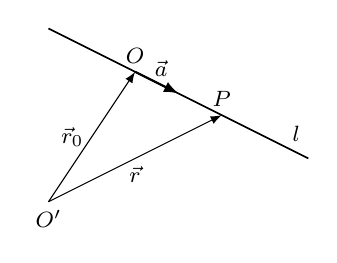
\begin{tikzpicture}[scale=1.1]
        \footnotesize
        \coordinate (O) at (0, 0);
        \coordinate (A) at (1, 1.5);
        \coordinate (B) at (2, 1);
        \coordinate (C) at (1.5, 1.25);
        \coordinate (L1) at (0, 2);
        \coordinate (L2) at (3, 0.5);


        \draw[-latex] (O) -- (A);
        \draw[-latex] (O) -- (B);
        \draw[thick, -latex] (A) -- (C);

        \draw[semithick] (L1) -- (L2);

        \point (O);
        \point (A);
        \point (B);

        \draw (O) node[anchor=north]{$O'$};
        \draw (A) node[anchor=south]{$O$};
        \draw (B) node[anchor=south]{$P$};

        \draw (1, 0.5) node[anchor=north]{$\vec{r}$};
        \draw (0.5, 0.75) node[anchor=east]{$\vec{r}_0$};
        \draw (1.3, 1.35) node[anchor=south]{$\vec{a}$};
        \draw (3, 0.6) node[anchor=south east]{$l$};
    \end{tikzpicture}
    \caption{}
    \label{pic:math-line}
\end{wrapfigure}
Рассмотрим необходимое условие, чтобы произвольная точка~$P$ с радиус-вектором~$\vec{r}$ лежала на прямой~$l$, проходящей через точку~$O$ с радиус вектором $\vec{r}_0$ (\lookPicRef{pic:math-line}). Пусть $ \vec{a} = \begin{pmatrix} a_1 & \cdots & a_n\end{pmatrix}^{\T}$~--- направляющий вектор прямой $l$, то есть $l$ параллельна прямой, содержащей вектор $\vec{a}$, тогда формально данное условие можно записать так:
\begin{equation}
    \vec{r} = \vec{r}_0 + \lambda \vec{a},\quad \lambda \in \R.
\end{equation}
Конкретизируем для случая векторов из $\R^2$:
\begin{gather*}
    \vec{r} - \vec{r}_0 = \lambda \vec{a} \quad \Rightarrow \quad
    \begin{cases}
        x - x_0 = \lambda x_a,\\
        y - y_0 = \lambda y_a.
    \end{cases}
\end{gather*}
Решив данную систему уравнений, получим, что
\begin{equation*}
    \lambda = \frac{x - x_0}{x_a} = \frac{y - y_0}{y_a}.
\end{equation*}
преобразуем второе равенство:
\begin{gather*}
    \frac{1}{x_a} \cdot x + \left( - \frac{1}{y_a} \right) \cdot y + \left( \frac{y_0}{y_a} - \frac{x_0}{x_a} \right) = 0,\\
    y_a x + (-x_a)y + (x_a y_0 - y_a x_0) = 0,
\end{gather*}
Сделав замену $y_a \equiv A$, $-x_a \equiv B$, $x_a y_0 - y_a x_0 \equiv C$, получим \imp{каноническое уравнение прямой на плоскости в декартовых координатах}:
\begin{equation}
    Ax + By + C = 0.
\end{equation}
Заметим, что
\begin{equation*}
    \scalar{a}{n} \equiv \scalar{a}{
    \begin{pmatrix}
        A\\
        B
    \end{pmatrix}} = x_a y_a - y_a x_a = 0,
\end{equation*}
значит, $\vec{n} \perp \vec{a}$, то есть вектор $\vec{n}$ есть вектор нормали к прямой с направляющим вектором $\vec{a}$, так как коэффициенты $A$ и $B$ не зависят от фиксированной точки $O$.

\subsection{Плоскость}

\begin{wrapfigure}{r}{0.35\tw}
    \centering
    \vspace{-1pc}
    \tikzsetnextfilename{math-plane}
    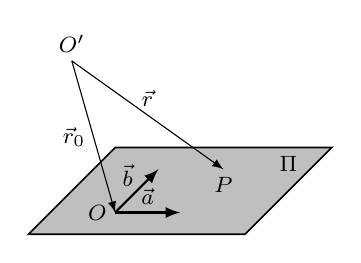
\begin{tikzpicture}[scale=1.1]
        \footnotesize

        \draw[semithick, fill=lightgray] (1, -1) -- (3.5, -1) -- (2.5, -2) -- (0, -2) -- cycle;

        \coordinate (O) at (0.5, 0);
        \coordinate (A) at (1, -1.75);
        \coordinate (B) at (2.25, -1.25);
        \coordinate (C) at (1.75, -1.75);
        \coordinate (D) at (1.5, -1.25);


        \draw[-latex] (O) -- (A);
        \draw[-latex] (O) -- (B);

        \draw[thick, -latex] (A) -- (C);
        \draw[thick, -latex] (A) -- (D);

        \point (O);
        \point (A);
        \point (B);

        \draw (O) node[anchor=south]{$O'$};
        \draw (A) node[anchor=east]{$O$};
        \draw (B) node[anchor=north]{$P$};

        \draw (1.375, -0.625) node[anchor=south]{$\vec{r}$};
        \draw (0.75, -0.875) node[anchor=east]{$\vec{r}_0$};
        \draw (1.375, -1.75) node[anchor=south]{$\vec{a}$};
        \draw (1.3, -1.55) node[anchor=south east]{$\vec{b}$};
        \draw (3.2, -1) node[anchor=north east]{$\Pi$};

    \end{tikzpicture}
    \caption{}
    \label{pic:math-plane}
\end{wrapfigure}
Аналогично предыдущему разделу, рассмотрим условие принадлежности точки $P$ с радиус-вектором $\vec{r}$ плоскости $\Pi$ в $\R^3$. Пусть неколлинеарные ($ \cross{a}{b} \not = 0$) векторы  $\vec{a}$ и $\vec{b}$~--- направляющие векторы плоскости $\Pi$, а точка $O$ с радиус-вектором $\vec r_0$ такова, что $\vec{r}_0 \in \Pi$. Тогда
\begin{equation}
    \vec{r} = \vec{r}_0 + \lambda\vec{a} + \mu\vec{b} \quad \Rightarrow \quad \begin{cases}
    x - x_0 = \lambda x_a + \mu x_b,\\
    y - y_0 = \lambda y_a + \mu y_b,\\
    z - z_0 = \lambda z_a + \mu z_b;
\end{cases}\quad \lambda, \mu \in \R.
\end{equation}
Преобразуем полученную систему уравнений:
\begin{align*}
& \left\{
\begin{aligned}
    \lambda &= \dfrac{x - x_0 - \mu x_b}{x_a},\\
    y - y_0 &= \dfrac{x - x_0 - \mu x_b}{x_a} \cdot y_a + \mu y_b,\\
    z - z_0 &= \lambda z_a + \mu z_b.
\end{aligned}\right.\\
& \left\{
\begin{aligned}
    \lambda &= \dfrac{x - x_0 - \mu x_b}{x_a},\\
    y - y_0 &= (x - x_0) \cdot \dfrac{y_a}{x_a} + \mu \left(y_b - \dfrac{x_b y_a}{x_a} \right),\\
    z - z_0 &= \lambda z_a + \mu z_b.
\end{aligned}\right.\\
&\left\{
\begin{aligned}
    \lambda &= \dfrac{x - x_0 - \mu x_b}{x_a},\\
    \mu &= \dfrac{x_a y - x_a y_0 - (x - x_0) \cdot y_a}{x_a y_b - x_b y_a},\\
    z - z_0 &= \lambda z_a + \mu z_b.
\end{aligned}\right.
\end{align*}
Подставим выражения для $\lambda$ и $\mu$ в третье уравнение:
\begin{multline*}
    z - z_0 = \dfrac{x - x_0 - \mu x_b}{x_a} \cdot z_a + \mu z_b = (x - x_0) \cdot \dfrac{z_a}{x_a} + \mu \left( z_b - \dfrac{x_b z_a}{x_a} \right) = \\
    = (x - x_0) \cdot \dfrac{z_a}{x_a} + \dfrac{x_a y - x_a y_0 - (x - x_0) \cdot y_a}{x_a y_b - x_b y_a} \cdot \left( z_b - \dfrac{x_b z_a}{x_a} \right)
\end{multline*}
Приведя подобные слагаемые с $x$, $y$ и $z$, получим:
\begin{multline*}
z = x \cdot \underbrace{\left( \dfrac{z_a}{x_a} - \dfrac{y_a}{x_a y_b - x_b y_a} \left( z_b - \dfrac{x_b z_a}{x_a} \right) \right)}_A +\\
+ y \cdot \underbrace{\dfrac{x_a}{x_a y_b - x_b y_a} \cdot \left( z_b - \dfrac{x_b z_a}{x_a} \right)}_B +\\
+ \underbrace{z_0 - \dfrac{x_0 z_a}{x_a} - \dfrac{x_a y_0 - x_0 y_a}{x_a y_b - x_b y_a} \cdot \left( z_b - \dfrac{x_b z_a}{x_a} \right)}_D.
\end{multline*}
Сделаем замену:
\begin{align*}
&
\begin{aligned}
    A \equiv  \dfrac{z_a}{x_a} &- \dfrac{y_a}{x_a y_b - x_b y_a} \left( z_b - \dfrac{x_b z_a}{x_a} \right) = \\
    &\quad\quad= \frac{x_a y_b z_a - x_b y_a z_a}{x_a (x_a y_b - x_b y_a)} - \frac{x_a y_a z_b - x_b y_a z_a}{x_a (x_a y_b - x_b y_a)} = \frac{y_b z_a - y_a z_b}{x_a y_b - x_b y_a},
\end{aligned}\\
&
B \equiv \dfrac{x_a}{x_a y_b - x_b y_a} \cdot \left( z_b - \dfrac{x_b z_a}{x_a} \right) 
%= \frac{x_a (x_a z_b - x_b z_a)}{x_a (x_a y_b - x_b y_a)} = 
\frac{x_a z_b - x_b z_a}{x_a y_b - x_b y_a},\\
&
D \equiv z_0 - \dfrac{x_0 z_a}{x_a} - \dfrac{x_a y_0 - x_0 y_a}{x_a y_b - x_b y_a} \cdot \left( z_b - \dfrac{x_b z_a}{x_a} \right).
\end{align*}
В результате такой замены получим уравнение
\begin{equation}
Ax + By - z + D = 0.
\end{equation}
Домножим в нём обе части на $\xi \equiv x_a y_b - x_b y_a$ и сделаем ещё одну замену:
\begin{equation*}
A'x + B'y + C'z + D' = 0,
\end{equation*}
где $D' = \xi D$, а
\begin{equation*}
\begin{cases}
    A' = y_b z_a - y_a z_b = \det
    \begin{pmatrix}
        y_b & z_b\\
        y_a & z_a
    \end{pmatrix}\\[1pc]
    B' = x_a z_b - x_b z_a = \det
    \begin{pmatrix}
        x_a & z_a\\
        x_b & z_b
    \end{pmatrix}\\[1pc]
    C' = x_b y_a - x_a y_b = \det
    \begin{pmatrix}
        x_b & y_b\\
        x_a & y_a
    \end{pmatrix}
\end{cases}
\end{equation*}
Легко видеть, что
\begin{equation}
\begin{pmatrix}
    A'\\
    B'\\
    C'
\end{pmatrix} =
\cross{b}{a} \equiv \vec{n}.
\end{equation}
Из свойств векторного произведения вектор $\vec n$ является \imp{вектором нормали} к плоскости $\Pi$.

Теперь  самое первое условие можно записать так:
\begin{equation}
\scalar{r}{n} = \triple{r}{b}{a} = -D' = (\vec{r}_0, \vec{b}, \vec{a}).
\end{equation}

\subsection{Производная}

\begin{wrapfigure}[11]{r}{0.46\tw}
	\centering
	\vspace{-1.1pc}
	\centering
	\begin{tikzpicture}[scale=1.1]
		\footnotesize
		
%		\foreach \x in {-0.5, -0.4,...,3} {
%			\draw [line width=.1pt] (\x, -0.5) -- (\x, 3);
%		};
%		
%		\foreach \x in {0, 1,...,3} {
%			\draw [line width=.4pt] (\x , -0.5) -- (\x , 3);
%		};
%		
%		\foreach \y in {0, 1,...,3} {
%			\draw [line width=.4pt] (-0.5, \y) -- (3, \y);
%		};
%		
%		\foreach \y in {-0.5, -0.4,...,3} {
%			\draw [line width=.1pt] (-0.5, \y) -- (3, \y);
%		};
		
		\draw[semithick, -latex] (-0.5, 0) -- (3, 0); 		
		\draw[semithick, -latex] (0, -0.5) -- (0, 3); 	
		
		\draw [thick] (-0.3, 0.5) .. controls (2, 0.5) and (2, 3) .. (3, 3);	
		
		\draw (0.5, 0.28) -- (2.5, 2.28);
		\draw [dashes] (0, 1.2) -- (2.6, 1.2);
		\draw [dashes] (0, 2.5) -- (2.6, 2.5);
		\draw [dashes] (1.4, 0) -- (1.4, 1.6);
		\draw [dashes] (2.3, 0) -- (2.3, 2.9);
		\draw [latex-latex] (2.3, 1.2) -- (2.3, 2.08);
		
		\draw (1.8, 1.2) arc(0:43:0.4);
		
		\draw (1.8, 1.4) node[anchor=west]{$\alpha$};
		\draw (3, 0) node[anchor=south]{$x$};
		\draw (0, 3) node[anchor=west]{$f(x)$};
		\draw (1.4, -0.06) node[anchor=north]{$x_0$};
		\draw (2.3, 0) node[anchor=north]{$x_0 + \Delta x$};
		\draw (0, 1.2) node[anchor=east]{$f(x_0)$};
		\draw (0, 2.5) node[anchor=east]{$f(x + \Delta x)$};
		\draw (2.3, 1.6) node[anchor=west]{$df(x_0)$};
		
		
		\draw [fill=white] (1.4, 1.2) circle(0.03);
		\draw [fill=white] (2.3, 1.2) circle(0.03);
		\draw [fill=white] (2.3, 2.5) circle(0.03);
		\draw [fill=white] (1.4, 0) circle(0.03);
		\draw [fill=white] (2.3, 0) circle(0.03);
		\draw [fill=white] (2.3, 2.08) circle(0.03);
		\draw [fill=white] (0, 1.2) circle(0.03);
		\draw [fill=white] (0, 2.5) circle(0.03);
	\end{tikzpicture}
	\caption{}
	\label{pic:math-div}
\end{wrapfigure}
\term{Производная в точке}~--- предел отношения приращения функции к приращению её аргумента при стремлении приращения аргумента к нулю, если такой предел существует. \imp{Геометрический смысл производной}: значение производной в точке численно равно тангенсу угла наклона касательной к графику функции в данной точке. Следовательно, точки, где производная обнуляется, соответствуют локальным минимумам и максимумам функции.
\begin{equation}
	f^\prime(x_0) = \lim_{\Delta x \to 0}\frac{f(x_0 + \Delta x) - f(x_0)}{\Delta x}
\end{equation}
Общепринятые обозначения для производной функции $f(x)$ в точке $x_0$:
\begin{equation}
	f^\prime(x_0) = f^\prime_x(x_0) = D f(x_0) = \frac{d f}{d x}(x_0) = \dot{f} (x_0).
\end{equation}
Правила дифференцирования:\\[-0.5pc]
\begin{minipage}{0.5\textwidth}
	\begin{align*}
		(f+g)^\prime &= f^\prime + g^\prime;\\
		(Cf)^\prime &= Cf^\prime;\\
		(fg)^\prime &= f^\prime g + f g^\prime;
	\end{align*}
\end{minipage}
\begin{minipage}{0.5\textwidth}
	\begin{align*}
		\left(\dfrac{f}{g}\right)^\prime &= \dfrac{f^\prime g - f g^\prime}{g^2};\\
		\dfrac{d}{dx}f\bigl(g(x)\bigr) &= \dfrac{df(g)}{dg}\dfrac{dg(x)}{dx}.
	\end{align*}
\end{minipage}\\[0.5pc]
Таблица производных:
\begin{align*}
	(x^a)^\prime &= a x^{a-1};
	& (\cos x)^\prime &= - \sin x;
	& (\arccos x)^\prime &= - \dfrac{1}{\sqrt{1 - x^2}};\\
	(a^x)^\prime &= a^x \ln a;
	& (\log_a x)^\prime &= \dfrac{1}{x \ln a};
	& (\arctg x)^\prime &= \dfrac{1}{1 + x^2};\\
	(\sin x)^\prime &= \cos x;
	& (\arcsin x)^\prime &=
	\dfrac{1}{\sqrt{1 - x^2}};
	&  (\arcctg x)^\prime &= - \dfrac{1}{1 + x^2}.
\end{align*}

\subsection{Интеграл}
\term{Неопределенным интегралом} функции $f(x)$ называется такая функция $F(x)$, производная которой равна $f(x)$.
\begin{equation}
	F(x) = \int f(x)dx,\quad F^\prime(x)=f(x).
\end{equation}

\begin{wrapfigure}{r}{0.46\tw}
	\centering
	\vspace{-1.1pc}
	\centering
	\begin{tikzpicture}[scale=1.1, yscale=0.7]
		\footnotesize
		\clip(-0.5, -1.05) rectangle (3.6, 2.1);
		
%		\foreach \x in {-5, -4.9,...,5} {
%			\draw [line width=.1pt] (\x, -5) -- (\x, 5);
%		};
%		
%		\foreach \x in {-5, -4,..., 5} {
%			\draw [line width=.4pt] (\x , -5) -- (\x , 5);
%		};
%		
%		\foreach \y in {-5, -4,..., 5} {
%			\draw [line width=.4pt] (-5, \y) -- (5, \y);
%		};
%		
%		\foreach \y in {-5, -4.9,..., 5} {
%			\draw [line width=.1pt] (-5, \y) -- (5, \y);
%		};
		

		\fill [lightgray] (0.4, 0) -- (0.4, 1.7) .. controls (0.9, 1.65) and (1.1, 0.85) .. (1.55, 0) -- cycle;	
		\fill [lightgray] (1.55, 0) .. controls (1.9, -0.9) and (2.3, -1.2) .. (2.5, -0.8) -- (2.5, 0) -- cycle;	
		\draw [thick] (-0.3, 0.5) .. controls (1, 5) and (2, -5) .. (3, 1);	
		
		\draw[semithick, -latex] (-0.5, 0) -- (3.5, 0); 		
		\draw[semithick, -latex] (0, -0.5) -- (0, 2); 
		
		\draw [dashes] (0.4, 0) -- (0.4, 1.7);
		\draw [dashes] (2.5, 0) -- (2.5, -0.8);

		\draw (0.9, 0.5) node{$S_+$};
		\draw (2.15, -0.45) node{$S_-$};
		\draw (3.5, 0) node[anchor=south]{$x$};
		\draw (0, 2) node[anchor=west]{$y$};
		\draw (0.4, 0) node[anchor=north]{$a$};
		\draw (2.5, 0) node[anchor=south]{$b$};
		\draw (2.95, 0.8) node[anchor=west]{$f(x)$};

		\point (0.4, 1.7);
		\point (0.4, 0);
		\point (2.5, 0);
		\point (2.5, -0.8);
		
	\end{tikzpicture}
	\caption{}
	\label{pic:math-int}
\end{wrapfigure}
\term{Определенный интеграл} характеризуется верхним и нижним пределом интегрирования. Значение определенного интеграла численно равно площади под графиком функции на данном промежутке и вычисляется по формуле \imp{Ньютона--Лейбница}:
\begin{equation}
	\int\limits^b_a f(x) \,d x = F(x) \biggr|^b_a = F(b) - F(a)
\end{equation}
Правила интегрирования:
\begin{align*}
	&\int c f(x) \,d x = c \int f(x) \,d x;\quad &&  \int f(ax + b) \,d x = \dfrac{1}{a}F(ax + b) + C;\\
	&\int f \,d g = fg - \int g \,d f; && \int \bigl[f(x) + g(x)\bigr] \,d x = \int f(x) \,d x + \int g(x) \,d x;
\end{align*}
Таблица интегралов:
\begin{align*}
	&\int  x^a \,d x = \dfrac{x^{a+1}}{a+1} + C,\quad a \neq -1; \quad
	&&\int \dfrac{dx}{\sqrt{a^2 - x^2}} = \arcsin\dfrac{x}{a} + C;\\
	&\int \frac{dx}{x} = \ln x + C;
	&&\int \dfrac{dx}{-\sqrt{a^2 - x^2}} = \arccos\dfrac{x}{a} + C;\\
	&\int a^x \,d x = \dfrac{a^x}{\ln a} + C;
	&&\int \dfrac{dx}{x^2 + a^2} = \dfrac{1}{a} \arctg \dfrac{x}{a} + C; \\
	&\int \cos x \,d x = \sin x + C;
	&&\int \dfrac{dx}{x^2 - a^2} = \dfrac{1}{2a} \ln \dfrac{|x - a|}{|x + a|} + C;\\
	&\int \sin x \,d x = -\cos x + C;
	&&\int \dfrac{dx}{\sqrt{x^2 + a}} = \ln \left| x + \sqrt{x^2 + a} \right| + C.
\end{align*}

Рассмотрим пример использования интеграла~--- получим формулу для нахождения объема шара с радиусом~$R$. Сначала получим вспомогательную формулу площади круга радиуса~$R$. Для этого рассмотрим тонкое кольцо радиуса~$r$~и ширины~$dr$, его площадь составляет~$2\pi r \,d r$. Следовательно, интегрируя площадь таких колец по радиусу~$r$ от~$0$ до~$R$, получим площадь круга
\begin{equation*}
    S = \int_0^R 2 \pi r \,d r = 2 \pi \cdot \left.\frac{r^2}{2} \right|_0^R = \pi R^2.
\end{equation*}
Теперь, используя полученное выражение для площади круга, легко найти объем шара. Рассмотрим тонкий слой толщины~$dx$ на расстоянии~$x$ от центра шара, его радиус равен $\sqrt{R^2 - x^2}$. Проинтегрируем объем таких слоев~по~$x$ от~$-R$ до~$R$:
\begin{equation*}
    V 
        = \int_{-R}^{R} \pi (R^2 - x^2) \,d x 
        = \pi \left.\left(xR^2 - \frac{x^3}{3}\right)\right|_{-R}^{R}
        = \pi \left(2R^3 - \frac{2R^3}{3} \right) 
        = \frac{4}{3} \pi R^3.
\end{equation*}
\subsection{Телесный угол}
\label{subsec:solid-angle}

\begin{wrapfigure}{r}{0.46\tw}
	\centering
	\vspace{-1.1pc}
	\centering
	\begin{tikzpicture}[scale=1.1]
		\footnotesize
%		\clip(-2.1, -2.1) rectangle (2.1, 2.1);
%		
%		\foreach \x in {-5, -4.9,...,5} {
%			\draw [line width=.1pt] (\x, -5) -- (\x, 5);
%		};
%		
%		\foreach \x in {-5, -4,..., 5} {
%			\draw [line width=.4pt] (\x , -5) -- (\x , 5);
%		};
%		
%		\foreach \y in {-5, -4,..., 5} {
%			\draw [line width=.4pt] (-5, \y) -- (5, \y);
%		};
%		
%		\foreach \y in {-5, -4.9,..., 5} {
%			\draw [line width=.1pt] (-5, \y) -- (5, \y);
%		};

		
		\draw [semithick] (0, 0) circle (2);
		\draw [semithick] (-2, 0) arc(-180:0:2 and 0.5);
		\draw [semithick, dashes] (-2, 0) arc(180:0:2 and 0.5);
		
		\draw [top color=white!80!black, bottom color=white!50!black] (0, 0.8) .. controls +(270:0.1) 
		and ++(0:-0.1) .. (0.2, 0.6) .. controls ++(0:0.2) 
		and ++(0:-0.2) .. (0.6, 0.8) .. controls ++(0:0.1) 
		and ++(0:-0.1) .. (0.9, 0.6) .. controls +(0:0.1) 
		and ++(270:0.2) .. (1.1, 0.8) .. controls +(90:0.2) 
		and ++(0:0.1) .. (0.9, 1.2) .. controls +(180:0.1) 
		and ++(0:0.1) .. (0.6, 1.1) .. controls +(180:0.1) 
		and ++(0:0.1) .. (0.3, 1.4) .. controls +(180:0.2) 
		and ++(90:0.2) .. (0, 0.8) -- cycle;

		
		\draw [-latex] (0, 0) -- (-2, 0);
		\draw [top color=white!80!black, bottom color=white!50!black] (0, 0.8) .. controls +(270:0.1) 
		and ++(0:-0.1) .. (0.2, 0.6) .. controls ++(0:0.2) 
		and ++(0:-0.2) .. (0.6, 0.8) .. controls ++(0:0.1) 
		and ++(0:-0.1) .. (0.9, 0.6) .. controls ++(0:0.1)
		and ++(225:0.01) ..(1.03, 0.62) -- (0, 0) -- cycle;

		
		\draw (0.7, 0.95) node{$S$};
		\draw (-1, 0) node[anchor=south]{$R$};
		\draw (0, 0) node[anchor=north west]{$O$};
		\draw [fill=white] (0, 0) circle(0.03);
		
	\end{tikzpicture}
	\caption{}
	\label{pic:math-solid-angle}
\end{wrapfigure}
\term{Телесный угол}~--- часть пространства, которая является объединением всех лучей, выходящих из данной точки (вершины угла) и пересекающих некоторую поверхность (которая называется поверхностью, стягивающей данный телесный угол). Телесный угол измеряется в стерадианах и равен отношению площади сферы, которую вырезает данный угол, к квадрату радиуса данной сферы.
\begin{equation}
	\Omega = \frac{S}{R^2}
\end{equation}
Телесный угол полной сферы равен $4\pi$. Величину телесного угла, образованного конусом с углом раствора $\alpha$ можно определить по формуле
\begin{equation}
	\Omega = 2 \pi \left(1 - \cos \frac{\alpha}{2}\right).
\end{equation}

Телесный угол, соответствующий сегменту сферы радиуса $R$ и высоты $h$, равен
\begin{equation}
	\Omega = 2 \pi \left(1 - \dfrac{h}{\sqrt{R^2 + h^2}}\right).
\end{equation}

Для сферического треугольника с углами $\alpha$, $\beta$ и $\gamma$ справедливо соотношение
\begin{equation}
	\Omega = \alpha + \beta + \gamma - \pi
\end{equation}

\subsection{Формулы приближенного вычисления}
Формулы приближенного вычисления при $x \ll 1$:
\begin{align*}
	\sin x &\approx x - \frac{x^3}{6} \approx x & \cos x &\approx 1 - \frac{x^2}{2} \\
	\tg x &\approx x & \ln(1+x) &\approx x \\
	(1 + x)^\alpha &\approx 1 + \alpha x & e^x &\approx 1 + x \\
	\sin (\theta + x) &\approx \sin \theta + x \cos \theta & \cos(\theta + x) &\approx \cos \theta - x \sin \theta
\end{align*}

\begin{wrapfigure}{r}{0.5\tw}
	\centering
	\vspace{-.9pc}
	\begin{tikzpicture}
		\begin{axis}[
			width	=	.5\tw,
			height	=	4.5cm,
			xlabel	=	{$x$},
			ylabel	=	{$y$},
%			extra x ticks	=	{1.571},
%			ytick = {-20, -10, 0, 10, 20},
			ymax	=	1,
			ymin	=	0,
			xmax	=	1.571,
			xmin	=	0,
%			xtick	=	{0, 4, 8, 12, 16, 20, 24},
%			x dir = reverse
			legend cell align=left,
				legend style={
				row sep = 1mm,
				draw=none,
				fill=none,
				font=\scriptsize,
				at={(axis cs:1.5, 0.1)}, anchor=south east,
				},
			]
			\addplot [domain=0:2, samples=100] {sin(deg(x))};
			\addplot [domain=0:2, samples=100, dashed] {x};
			\addplot [domain=0:2, samples=100, dotted] {x - (x^3)/6};
			\legend{
				$\sin(x)$,
				$x$,
				$x - x^3\!/6$
			}
		\end{axis}
	\end{tikzpicture}
	\caption{}
\end{wrapfigure}
Также существует равенство для нескольких малых переменных:
\begin{equation*}
	(1 + a)^\alpha (1 + b)^\beta \ldots \approx 1 + \alpha a + \beta b + \ldots
\end{equation*}

\input{sections/maths/harmony.tex}
